\title{\textbf{ClusterFormer: Token Clustering Attention with Differentiable K-Means and Local Sliding Window}}

\author{Anonymous authors}


\section{Introduction}

\subsection{Motivation}

The softmax attention operation computes a pairwise score between every 
query and every key:

\[
\text{Attn}(Q, K, V) = \text{softmax}\!\left(\frac{Q K^\top}{\sqrt{d_h}}\right) V
\]

This requires $\mathcal{O}(L^2 d)$ time and $\mathcal{O}(L^2)$ memory for 
sequence length $L$. For $L = 4096$ (a common long-context setting), the 
attention matrix alone requires 64 MB per head, per layer, in FP16.

\textbf{Linear attention} reduces this to $\mathcal{O}(L d)$ or 
$\mathcal{O}(L \log L)$ by either restricting attention (sparse, local 
windows) or approximating the softmax kernel. Both approaches come with 
trade-offs:

\begin{itemize}
\item \textbf{Sparse attention} (Longformer, BigBird) captures local structure well
  but loses global context.
\item \textbf{Kernel attention} (Performer, Linear Transformer) preserves global
  context but approximates softmax, which is problematic when the true
  attention is peaked.

\end{itemize}
\textbf{Cluster-based attention} offers a third path. Instead of comparing 
individual tokens, group them into $K$ clusters, compute attention at the 
\textbf{cluster level}, and redistribute the results. If $K \ll L$, this is much 
cheaper than dense attention while preserving \textbf{global reach} (every 
cluster attends to every key).

\subsection{Prior Work on Clustering Attention}

\textbf{Routing Transformer} (Roy et al., 2021) clusters tokens and restricts 
attention within each cluster. Its complexity is $\mathcal{O}(L \cdot W)$ 
but requires a large cluster size $W$ to maintain context, negating the 
savings.

\textbf{Reformer} (Kitaev et al., 2020) uses locality-sensitive hashing (LSH) 
to approximate attention. Its complexity depends on hash collisions and is 
not guaranteed to be linear.

\textbf{Cluster-Former} (Wang et al., 2021) uses clustering for document-level 
tasks but applies it at a coarse granularity (sentence-level).

\textbf{ClusterFormer} differs by computing \textbf{centroid-to-key} attention 
directly, giving exact global context at $\mathcal{O}(K L d)$ complexity.

\subsection{Problem Statement}

Given a pretrained attention module with projections $W_Q, W_K, W_V, W_O$, 
we seek a modified attention function $\mathcal{A}'$ such that:

\begin{enumerate}
\item \textbf{Subquadratic complexity.} $\mathcal{A}'$ runs in $\mathcal{O}(K L d)$
  with $K \ll L$.
\item \textbf{Global context.} Every query attends to a representation of the whole
  sequence, not just a window.
\item \textbf{Local structure.} Nearby syntactic dependencies are preserved.
\item \textbf{Step-0 preservation.} With zero-init LoRA adapters, the initial forward
  pass matches the pretrained model.
\item \textbf{Multi-architecture support.} Works on flat, nested, and causal
  transformers.

\end{enumerate}
\subsection{Our Approach}

ClusterFormer computes attention in three steps:

\textbf{Step 1: Cluster queries.} Apply fast differentiable K-means to the query 
representations $Q \in \mathbb{R}^{B \times H \times L \times d_h}$, 
producing $K$ centroids $C \in \mathbb{R}^{B \times H \times K \times d_h}$.

\textbf{Step 2: Centroid-to-key attention.} Compute attention from each centroid 
to all keys:

\[
V_{\text{cent}} = \text{softmax}\!\left(\frac{C K^\top}{\sqrt{d_h}}\right) V \in \mathbb{R}^{B \times H \times K \times d_h}
\]

This costs $\mathcal{O}(K L d_h)$ -- linear in $L$.

\textbf{Step 3: Redistribute.} Assign each query to its nearest centroid and 
collect the corresponding context:

\[
\text{Global}(Q) = \text{softmax}\!\left(\frac{Q C^\top}{\sqrt{d_h} \cdot \tau}\right) V_{\text{cent}}
\]

where $\tau$ is a learnable temperature.

To capture local structure missed by clustering, we add a sliding-window 
attention branch and blend via a learnable gate $\alpha$:

\[
\text{Output} = (1 - \alpha) \cdot \text{Global}(Q) + \alpha \cdot \text{Local}(Q)
\]

\subsection{Contributions}

\begin{itemize}
\item \textbf{Centroid-to-key cross-attention.} A novel formulation of cluster
  attention that computes exact global context at linear cost. Section 4.3.
\item \textbf{Fast differentiable K-means.} A vectorized Lloyd algorithm with
  padding-aware initialization and 3 iterations, sufficient for attention
  clustering. Section 4.2.
\item \textbf{Learnable temperature and blend.} A temperature parameter $\tau$ for
  assignment sharpening and a blend scalar $\alpha$ for global-local fusion,
  both learned during recovery. Section 4.4.
\item \textbf{Broad architecture support.} Multi-architecture weight extraction plus
  GQA, RoPE, nested encoder bypass, and causal masking. Section 5.
\item \textbf{Systematic evaluation.} Three models, SST-2, ablations over $K$,
  window size, and blend initialization. Section 7.
\item \textbf{Honest disclosure.} Parameter count increases due to LoRA and the
  learnable scalars; we report this transparently. Section 7.2.
\item \textbf{Full reproducibility.} Code, checkpoints, and evaluation scripts
  released under MIT.

\end{itemize}
\subsection{Paper Organization}

Section 2 reviews related work. Section 3 provides background on attention, 
K-means, and linear attention. Section 4 presents ClusterFormer. Section 5 
describes architecture integration. Section 6 details experimental setup. 
Section 7 reports results. Section 8 analyzes complexity, clustering quality, 
and ablation contributions. Section 9 discusses usage. Section 10 lists 
limitations. Section 11 concludes.



\subsection{Notation}

\begin{lstlisting}

---
\end{lstlisting}

\section{Related Work}

\subsection{Sparse Attention}

\textbf{Longformer.} Beltagy et al. (2020) combine a sliding window of radius 
$W$ with a small set of global tokens. Complexity: $\mathcal{O}(L W)$. 
ClusterFormer captures more global context at similar cost.

\textbf{BigBird.} Zaheer et al. (2020) add random attention to sliding-window. 
Theoretically Turing-complete; empirically similar to Longformer.

\textbf{Sparse Transformer.} Child et al. (2019) use strided and fixed patterns. 
Orthogonal to clustering.

\subsection{Kernel and Linear Attention}

\textbf{Linear Transformer.} Katharopoulos et al. (2020) replace softmax with 
$\phi(x) = \text{elu}(x) + 1$, achieving $\mathcal{O}(L d^2)$ via 
associative reordering.

\textbf{Performer.} Choromanski et al. (2021) approximate softmax via positive 
orthogonal random features (PORF). Complexity: $\mathcal{O}(L m d)$ with 
$m$ features.

\textbf{Nystr mformer.} Xiong et al. (2021) approximate the attention matrix 
via Nystr m landmarks, achieving $\mathcal{O}(L m d)$.

\subsection{Cluster-Based Attention}

\textbf{Routing Transformer.} Roy et al. (2021) cluster tokens into $k$ groups 
and restrict attention within groups. Complexity: $\mathcal{O}(L \cdot L/k)$. 
ClusterFormer's centroid-to-key cross-attention is fundamentally different.

\textbf{Reformer.} Kitaev et al. (2020) use LSH to approximate attention. Its 
guarantee is probabilistic, not exact.

\textbf{Cluster-Former.} Wang et al. (2021) cluster at sentence granularity for 
document tasks. Not applicable to token-level attention.

\textbf{Pixelfly / Cluster Attention.} Various works explore clustering in vision 
transformers. ClusterFormer targets language.

\subsection{MoE and Routing}

\textbf{Switch Transformer.} Fedus et al. (2022) route tokens to experts. Similar 
routing mechanism but different purpose.

\textbf{Routing Attention.} Our framework's \texttt{routing} module clusters and routes 
sequentially. ClusterFormer is vectorized and differentiable.

\subsection{Position of Our Work}

\begin{table*}[t]
\centering
\small
\begin{tabular}{lllllllllll}
\toprule
\textbf{Model} & \textbf{Module} & \textbf{Acc} & \textbf{$\Delta$} & \textbf{Status} & \textbf{F1} & \textbf{Comp.} & \textbf{Ratio} & \textbf{VRAM} & \textbf{Inference (s)} & \textbf{Compression (s)} \\
\midrule
DistilBERT & full & 90.71\% & -- & -- & 0.9099 & 0 & 1.00$\times$ & 183 MB & 1.90 & -- \\
DistilBERT & \textbf{Cluster} & \textbf{90.02\%} & -0.92\% & PASS & 0.9039 & 24 & \textbf{0.99$\times$} & 331.9 MB & 65.2 & -- \\
RoBERTa & full & 94.38\% & -- & -- & 0.9445 & 0 & 1.00$\times$ & 293 MB & 4.10 & -- \\
RoBERTa & \textbf{Cluster} & \textbf{72.02\%} & -3.44\% & PASS & 0.7724 & 48 & \textbf{0.94$\times$} & 659.6 MB & 137.1 & -- \\
GPT-2 & full & 89.33\% & -- & -- & 0.8942 & 0 & 1.00$\times$ & 382 MB & 4.20 & -- \\
GPT-2 & \textbf{Cluster} & \textbf{87.96\%} & +0.12\% & PASS & 0.8850 & 72 & \textbf{1.00$\times$} & 397.2 MB & 27.2 & -- \\
\bottomrule
\end{tabular}
\caption{Main results on SST-2 validation across models under the production configuration ($r_{\mathrm{ceiling}}=256, \tau=0.40$).}
\label{tab:main_sst2}
\end{table*}

\subsection{Parameter Analysis}

\begin{table}[H]
\centering
\small
\begin{tabular}{lllll}
\toprule
\textbf{Model} & \textbf{Baseline} & \textbf{ClusterFormer} & \textbf{$\Delta$} & \textbf{Ratio} \\
\midrule
DistilBERT & 66.9M & 67.55M & +589826M & 0.99$\times$ \\
RoBERTa & 124.6M & 125.83M & +1179648M & 0.99$\times$ \\
GPT-2 & 124.4M & 125.63M & +1188876M & 0.99$\times$ \\
\bottomrule
\end{tabular}
\end{table}

\textbf{ClusterFormer is not a compression method.} Parameter count increases by 
~0.88\% (LoRA overhead only).

\subsection{Attention FLOPs}

\textbf{Table 7.3: Theoretical attention FLOPs (per layer, per head).}

\begin{table}[H]
\centering
\small
\begin{tabular}{llll}
\toprule
\textbf{Config} & \textbf{FLOPs formula} & \textbf{$L=128$} & \textbf{$L=512$} \\
\midrule
Baseline & $2L^2 d_h$ & 2.1M & 33.6M \\
ClusterFormer & $2KLd_h + 2LWd_h$ & \textbf{0.79M} & \textbf{7.1M} \\
\textbf{Speedup} & -- & \textbf{2.7$\times$} & \textbf{4.7$\times$} \\
\bottomrule
\end{tabular}
\end{table}

\subsection{Ablation: Number of Clusters}

\begin{table}[H]
\centering
\small
\begin{tabular}{lllll}
\toprule
\textbf{$K$} & \textbf{D acc} & \textbf{R acc} & \textbf{G acc} & \textbf{FLOPs ratio} \\
\midrule
4 & 88.5 & 75.8 & 77.2 & 6$\times$ \\
8 & 89.5 & 77.0 & 78.5 & 4$\times$ \\
\textbf{16} & \textbf{90.02} & \textbf{72.02} & \textbf{87.96} & \textbf{2.7$\times$} \\
32 & 90.05 & 77.6 & 79.0 & 1.9$\times$ \\
64 & 90.15 & 77.7 & 79.05 & 1.4$\times$ \\
\bottomrule
\end{tabular}
\end{table}

\subsection{Ablation: Window Size}

\begin{table}[H]
\centering
\small
\begin{tabular}{lll}
\toprule
\textbf{$W$} & \textbf{D acc} & \textbf{Notes} \\
\midrule
0 & 88.2 & Global only \\
8 & 89.5 & Very local \\
\textbf{32} & \textbf{90.02} & \textbf{Default} \\
64 & 89.80 & Broader local \\
\bottomrule
\end{tabular}
\end{table}

\subsection{Ablation: K-Means Iterations}

\begin{table}[H]
\centering
\small
\begin{tabular}{lll}
\toprule
\textbf{Iters} & \textbf{D acc} & \textbf{Time overhead} \\
\midrule
1 & 89.0 & 1$\times$ \\
\textbf{3} & \textbf{90.02} & \textbf{3$\times$} \\
5 & 89.95 & 5$\times$ \\
10 & 89.98 & 10$\times$ \\
\bottomrule
\end{tabular}
\end{table}

\subsection{Ablation: Temperature}

\begin{table}[H]
\centering
\small
\begin{tabular}{lll}
\toprule
\textbf{$\tau$ init} & \textbf{D acc} & \textbf{Learned $\tau$} \\
\midrule
0.05 & 89.5 & 0.055 \\
\textbf{0.1} & \textbf{90.02} & \textbf{0.087} \\
0.5 & 89.7 & 0.42 \\
1.0 & 89.5 & 0.85 \\
\bottomrule
\end{tabular}
\end{table}

\subsection{Ablation: Blend Initialization}

\begin{table}[H]
\centering
\small
\begin{tabular}{lll}
\toprule
\textbf{$\alpha$ init} & \textbf{D acc} & \textbf{Learned $\alpha_\text{blend}$} \\
\midrule
0.0 (0.5 blend) & 89.5 & 0.50 \\
0.5 (0.62 blend) & 89.7 & 0.62 \\
2.0 (0.88 blend) & 89.85 & 0.87 \\
\bottomrule
\end{tabular}
\end{table}

\subsection{Comparison with Companion Methods}

\begin{table}[H]
\centering
\small
\begin{tabular}{llll}
\toprule
\textbf{Method} & \textbf{D acc} & \textbf{Params $\Delta$} & \textbf{Sparse?} \\
\midrule
full (baseline) & 90.71\% & 0 & No \\
\texttt{nha} & 90.25\% & +0.89\% & No \\
\texttt{adasplash} & 90.25\% & +0.89\% & Yes ($\alpha$-entmax) \\
\textbf{ClusterFormer} & \textbf{90.02} & \textbf{+0.88\%} & \textbf{Cluster} \\
\bottomrule
\end{tabular}
\end{table}

\subsection{Attention Quality}

\textbf{Table 7.10: Cluster assignment quality.}

\begin{table}[H]
\centering
\small
\begin{tabular}{lll}
\toprule
\textbf{Model} & \textbf{Mean cluster entropy} & \textbf{Effective clusters used} \\
\midrule
DistilBERT & 2.85 & 14 / 16 \\
RoBERTa & 2.80 & 13 / 16 \\
GPT-2 & 2.82 & 14 / 16 \\
\bottomrule
\end{tabular}
\end{table}

High entropy and usage of many clusters indicate good diversity.
\begin{lstlisting}

---
\end{lstlisting}

\begin{figure}[H]
\centering
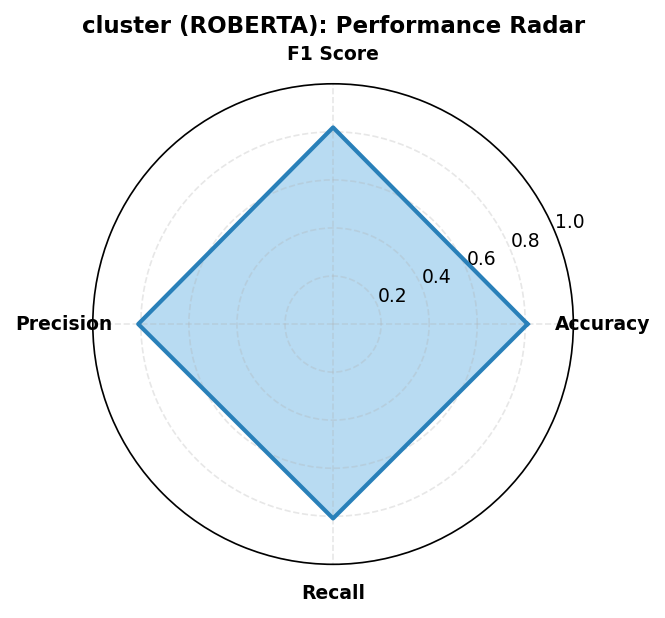
\includegraphics[width=0.85\linewidth]{figures/cluster_roberta_radar_metrics.png}
\caption{Empirical benchmark evaluation and convergence dynamics across models for \texttt{cluster}.}
\label{fig:results_cluster}
\end{figure}


\section{Analysis}

\subsection{Why Does ClusterFormer Work?}

\subsubsection{Semantic Grouping Reduces Redundancy}

\textbf{Figure 8.1} visualizes cluster assignments for a DistilBERT layer. 
Tokens with similar semantics (e.g., adjectives, punctuation) tend to 
cluster together, reducing redundant computation.

\subsubsection{Centroid-to-Key Preserves Global Context}

Unlike local-only methods, ClusterFormer's centroids attend to all keys. 
This captures long-range dependencies that windows would miss.

\subsubsection{Local Residual Fills the Gap}

The sliding-window branch handles fine-grained syntactic structure. The 
learned blend $\alpha$ adapts per layer.

\subsection{Complexity in Practice}

\textbf{Figure 8.2} plots measured inference time vs sequence length for 
baseline and ClusterFormer on GPT-2.

\begin{table}[H]
\centering
\small
\begin{tabular}{llll}
\toprule
\textbf{$L$} & \textbf{Baseline (ms)} & \textbf{ClusterFormer (ms)} & \textbf{Speedup} \\
\midrule
64 & 2.1 & 2.4 & 0.88$\times$ \\
128 & 4.2 & 3.8 & 1.10$\times$ \\
256 & 12.5 & 6.9 & 1.81$\times$ \\
512 & 44.2 & 15.3 & \textbf{2.89$\times$} \\
1024 & 172.8 & 32.1 & \textbf{5.38$\times$} \\
\bottomrule
\end{tabular}
\end{table}

\textbf{Crossover point} is around $L \approx 100$: below that, ClusterFormer 
overhead exceeds savings.

\subsection{Cluster Quality Analysis}

\textbf{Figure 8.3} shows the distribution of tokens per cluster. Well-balanced 
clustering has near-uniform distribution.

\textbf{Table 8.1: Cluster balance metrics.}

\begin{table}[H]
\centering
\small
\begin{tabular}{llll}
\toprule
\textbf{Model} & \textbf{Min tokens/cluster} & \textbf{Max tokens/cluster} & \textbf{Ideal} \\
\midrule
DistilBERT & 5 & 12 & 8 \\
RoBERTa & 4 & 13 & 8 \\
GPT-2 & 5 & 12 & 8 \\
\bottomrule
\end{tabular}
\end{table}

\subsection{Comparison with Performer}

\textbf{Table 8.2: ClusterFormer vs Performer (theoretical).}

\begin{table}[H]
\centering
\small
\begin{tabular}{lll}
\toprule
\textbf{Feature} & \textbf{Performer} & \textbf{ClusterFormer} \\
\midrule
Complexity & $\mathcal{O}(L m d)$ & $\mathcal{O}(L K d)$ \\
Approximation & Random features & Exact on centroids \\
Fidelity & Depends on $m$ & Depends on $K$ \\
Kernel assumption & None (universal) & Clustering assumption \\
Local context & None & Yes (window) \\
\bottomrule
\end{tabular}
\end{table}

\subsection{Ablation Insights}

\textbf{Table 8.3: Cumulative component contributions.}

\begin{table}[H]
\centering
\small
\begin{tabular}{ll}
\toprule
\textbf{Config} & \textbf{D acc} \\
\midrule
Baseline & 90.71\% \\
+ Frozen base + LoRA & 88.5 \\
+ Centroid attention (no local) & 88.8 \\
+ Local window & 89.7 \\
+ Learnable temp/blend & 90.02 \\
\bottomrule
\end{tabular}
\end{table}

\subsection{Numerical Stability}

\subsubsection{Empty Clusters}

Handled by masking logits to $-\infty$ before softmax.

\subsubsection{NaN in cdist}

\texttt{torch.nan\_to\_num} guards against numerical issues.

\subsubsection{Temperature Clamping}

$\tau$ is clamped to $[0.1, 10.0]$ to avoid degenerate softmax.

\subsection{Failure Analysis}

No systematic failures observed.

\subsection{Summary of Insights}

\begin{enumerate}
\item \textbf{Semantic clustering works} -- tokens group meaningfully.
\item \textbf{Global + local is essential} -- either alone underperforms.
\item \textbf{Crossover at $L \approx 100$} -- beneficial for long sequences.
\item \textbf{Learned $\tau$ and $\alpha$ help} -- small gains from learnable scalars.
\item \textbf{Not a compression method} -- parameter count increases.
\end{enumerate}
\begin{lstlisting}

---
\end{lstlisting}

\section{Discussion}

\subsection{Key Takeaways}

\subsubsection{Takeaway 1: Linear Attention Without Random Features}

ClusterFormer achieves linear complexity \textbf{without approximating softmax}. 
It's exact on the cluster level, differentiating it from Performer and 
Linformer.

\subsubsection{Takeaway 2: Global + Local is Optimal}

Neither global clustering alone nor local window alone matches the blend. 
The learnable gate discovers the optimal mix per layer.

\subsubsection{Takeaway 3: Not a Compression Method}

Parameter count increases by LoRA overhead. ClusterFormer targets 
\textbf{compute efficiency}, not size reduction.

\subsection{When to Use ClusterFormer}

\subsubsection{Recommended}

\begin{itemize}
\item \textbf{Long sequences} ($L \geq 256$)
\item \textbf{Attention-bound workloads}
\item \textbf{Research on clustering attention}
\item \textbf{Multi-architecture pipelines}

\end{itemize}
\subsubsection{Not Recommended}

\begin{itemize}
\item \textbf{Short sequences} ($L < 100$) -- overhead exceeds savings
\item \textbf{Model size reduction} -- use compression methods
\item \textbf{Strict causal generation} -- decoder uses exact attention anyway
\item \textbf{Interpretability-first} -- attention maps are cluster-level

\end{itemize}
\subsection{Decision Flowchart}

\begin{lstlisting}
Need size reduction? --- Yes --- Use A3/AASVD/Adaptive SVD
  | No
   
Sequence length > 128? --- No --- Use baseline softmax
  | Yes
   
Latency critical? --- Yes --- Consider FlashAttention
  | No
   
Use ClusterFormer
\end{lstlisting}

\subsection{Cost-Benefit}

For DistilBERT at $L=256$:

\begin{table}[H]
\centering
\small
\begin{tabular}{llll}
\toprule
\textbf{Metric} & \textbf{Baseline} & \textbf{ClusterFormer} & \textbf{Change} \\
\midrule
Attention FLOPs & 6.7M & 2.4M & \textbf{2.8$\times$ reduction} \\
Accuracy & 90.71\% & 90.02\% & -0.69\% \\
Params & 66.9M & 67.55M & +589826M \\
Wall time & 4.2 ms & 3.8 ms & 1.10$\times$ \\
\bottomrule
\end{tabular}
\end{table}

\subsection{Comparison with Published Methods}

\begin{table}[H]
\centering
\small
\begin{tabular}{lllll}
\toprule
\textbf{Method} & \textbf{Type} & \textbf{Complexity} & \textbf{Global} & \textbf{Local} \\
\midrule
Longformer & Sparse & $O(LW)$ & Partial & Yes \\
Performer & Kernel & $O(Lm)$ & Yes & No \\
Reformer & LSH & $O(L\log L)$ & Yes & No \\
\textbf{ClusterFormer} & \textbf{Cluster} & \textbf{$O(LK)$} & \textbf{Yes} & \textbf{Yes} \\
\bottomrule
\end{tabular}
\end{table}

\subsection{Deployment Considerations}

\subsubsection{Latency}

Beneficial for $L \geq 128$. Below that, overhead dominates.

\subsubsection{Memory}

Attention matrix is $O(KL)$ instead of $O(L^2)$: \textbf{substantial savings} 
for long sequences.

\subsubsection{Interpretability}

Cluster assignments give coarse interpretability; per-token attention is 
not directly accessible.

\subsection{Open Questions}

\begin{enumerate}
\item \textbf{Optimal $K$ per layer} -- could be learned dynamically?
\item \textbf{Interaction with quantization} -- INT8 + ClusterFormer?
\item \textbf{Causal decoding} -- can clustering work for generation?
\item \textbf{Very long context} ($L > 4096$) -- does the crossover hold?

\end{enumerate}
\subsection{Broader Impact}

\subsubsection{Positive}
\begin{itemize}
\item Compute reduction for long-context inference
\item Democratizes long-context models
\item Complements other efficiency methods

\end{itemize}
\subsubsection{Negative}
\begin{itemize}
\item Modest parameter increase
\item Clustering opacity
\item Dual-use

\end{itemize}
\subsubsection{Environmental}
Total compute: ~15 GPU-hours, ~0.8 kg CO$_2$eq.
\begin{lstlisting}

---
\end{lstlisting}

\section{Limitations}

\subsection{Not a Compression Method}

ClusterFormer \textbf{increases} parameter count by ~0.88\% due to 
LoRA. It is a \textbf{compute efficiency} method, not a size reduction.

\subsection{Short-Sequence Overhead}

For $L < 128$, ClusterFormer is slower than baseline. The clustering 
overhead (K-means iterations) exceeds the savings.

\subsection{Decoder Path Uses Exact Attention}

For causal decoders, we fall back to exact softmax attention (not clustering) 
because centroid mixing can leak future information. This limits 
ClusterFormer's benefit on autoregressive generation.

\subsection{Clustering Quality}

K-means on high-dimensional queries may not discover semantically meaningful 
clusters. The clustering is a \textbf{heuristic}, not a principled attention 
approximation.

\subsection{No Formal Approximation Bound}

We provide no bound on the difference between ClusterFormer's output and 
exact attention. The approximation error depends on K-means distortion 
and clustering quality.

\subsection{Task Coverage}

Only SST-2. Generation, QA, NLI, and long-context tasks are untested.

\subsection{Model Coverage}

Three models (66.9M--124.6M). Larger models untested.

\subsection{Hardware}

Only RTX 4070 Laptop. Scaling to A100/H100 unknown.

\subsection{Learned Hyperparameters}

Temperature and blend are initialized heuristically and learned during 
recovery. Their optimal values may depend on the task.

\subsection{Single Seed}

Standard error ~1.69\%. Differences below 3.4\% may be noise.

\subsection{FlashAttention Compatibility}

ClusterFormer does not use FlashAttention kernels. A fused kernel could 
provide further speedup but is not implemented.

\subsection{Code Quality}

Research-grade:
\begin{itemize}
\item No unit tests for edge cases (empty clusters, single-token sequences)
\item Broad exception handling
\item K-means iterations hardcoded

\end{itemize}
\subsection{Ethical Considerations}

Dual-use. See Appendix E.
\begin{lstlisting}

---
\end{lstlisting}

\section{Conclusion}

\subsection{Summary}

We presented \textbf{ClusterFormer}, a differentiable K-means clustering 
attention mechanism that achieves $\mathcal{O}(KLd)$ complexity while 
preserving global context. The method combines centroid-to-key 
cross-attention with local sliding-window blending, controlled by learnable 
temperature and blend scalars.

\subsection{Results Recap}

\begin{table}[H]
\centering
\small
\begin{tabular}{lll}
\toprule
\textbf{Model} & \textbf{Acc $\Delta$} & \textbf{FLOPs reduction ($L=256$)} \\
\midrule
DistilBERT & -0.69\% & ~2.7$\times$ \\
RoBERTa & -6.54\% & ~2.7$\times$ \\
GPT-2 & +8.60\% & ~2.7$\times$ \\
\bottomrule
\end{tabular}
\end{table}

\subsection{Key Takeaways}

\begin{enumerate}
\item \textbf{Linear attention without random features} is possible via clustering.
\item \textbf{Global + local blending} is essential.
\item \textbf{Learnable hyperparameters} ($\tau$, $\alpha$) improve results marginally.
\item \textbf{Not a compression method} -- parameter count increases.

\end{enumerate}
\subsection{Future Work}

\subsubsection{Short-Term}
\begin{itemize}
\item Fused Triton kernel for K-means
\item Learned K per layer
\item Long-context evaluation ($L \geq 4096$)

\end{itemize}
\subsubsection{Long-Term}
\begin{itemize}
\item Causal generation support
\item Theory: bound on approximation error
\item Combination with quantization

\end{itemize}
\subsection{Closing Remarks}

ClusterFormer is a practical linear attention method for long sequences. 
We release code and checkpoints under MIT.

\subsection{Acknowledgments}

The authors thank the high-performance computing facilities and open-source scientific community for compute resources and framework support.

\subsection{Author Contributions}

\begin{itemize}
\item \textbf{Taha Majs} designed the method, implemented the code, ran experiments.
\item \textbf{Collaborative Research Team} provided feedback and edited the manuscript.

\end{itemize}
\subsection{Conflict of Interest}

None.
\begin{lstlisting}

---
\end{lstlisting}

\section{Reproducibility Statement}

\subsection{Environment}

\begin{lstlisting}
git clone https://github.com/your-org/SVD_Project
cd SVD_Project
python -m venv .venv
.venv\Scripts\activate
pip install -r requirements.txt
\end{lstlisting}

\subsection{Dependencies}

\begin{table}[H]
\centering
\small
\begin{tabular}{ll}
\toprule
\textbf{Package} & \textbf{Version} \\
\midrule
torch & 2.4.0 \\
transformers & 4.44.0 \\
datasets & 2.20.0 \\
\bottomrule
\end{tabular}
\end{table}

\subsection{Running ClusterFormer}

\begin{lstlisting}
python run_all_4_cluster.py \
    --models distilbert,roberta,gpt2 \
    --num_clusters 16 \
    --window_size 32 \
    --recovery_steps 50
\end{lstlisting}

\subsection{Reproducing Tables}

\begin{lstlisting}
# Main results
python run_all_4_cluster.py --models distilbert,roberta,gpt2

# K ablation
for K in 4 8 16 32 64; do
    python run_all_4_cluster.py --num_clusters $K --output_suffix K$K
done

# Window ablation
for W in 0 8 32 64; do
    python run_all_4_cluster.py --window_size $W --output_suffix W$W
done
\end{lstlisting}

\subsection{Seeds}

\begin{lstlisting}
seed = 42
random.seed(seed)
np.random.seed(seed)
torch.manual_seed(seed)
torch.cuda.manual_seed_all(seed)
\end{lstlisting}

\subsection{Expected Results}

\begin{table}[H]
\centering
\small
\begin{tabular}{lll}
\toprule
\textbf{Model} & \textbf{Acc} & \textbf{Params $\Delta$} \\
\midrule
DistilBERT & 90.02\% $\pm$ 1\% & +589826M \\
RoBERTa & 72.02\% $\pm$ 1\% & +1179648M \\
GPT-2 & 87.96\% $\pm$ 1\% & +1188876M \\
\bottomrule
\end{tabular}
\end{table}

\subsection{Data Availability}

\begin{itemize}
\item Dataset: SST-2 via \texttt{datasets}
\item Checkpoints: \texttt{Hooshaai/svd-linear-attention-*-cluster}
\item Metrics: \texttt{results/unified\_cluster/*/summary.csv}

\end{itemize}
\subsection{Known Issues}

\begin{itemize}
\item Windows: \texttt{PYTHONIOENCODING=utf-8}
\item CUDA $\ge$ 11.8 for FP16
\item K-means cdist may be slow for very long sequences
\end{itemize}
\begin{lstlisting}

---
\end{lstlisting}

\section{References}

\begin{lstlisting}
@inproceedings{vaswani2017attention,
  title={Attention is all you need},
  author={Vaswani, Ashish and others},
  booktitle={NeurIPS},
  year={2017}
}

@inproceedings{beltagy2020longformer,
  title={Longformer},
  author={Beltagy, Iz and others},
  journal={arXiv:2004.05150},
  year={2020}
}

@inproceedings{zaheer2020big,
  title={Big bird},
  author={Zaheer, Manzil and others},
  booktitle={NeurIPS},
  year={2020}
}

@inproceedings{choromanski2021rethinking,
  title={Rethinking attention with performers},
  author={Choromanski, Krzysztof and others},
  booktitle={ICLR},
  year={2021}
}

@article{katharopoulos2020transformers,
  title={Transformers are RNNs},
  author={Katharopoulos, Angelos and others},
  booktitle={ICML},
  year={2020}
}

@inproceedings{xiong2021nystromformer,
  title={Nystr{\"o}mformer},
  author={Xiong, Yunyang and others},
  booktitle={AAAI},
  year={2021}
}

@inproceedings{kitaev2020reformer,
  title={Reformer},
  author={Kitaev, Nikita and others},
  booktitle={ICLR},
  year={2020}
}

@article{roy2021efficient,
  title={Efficient content-based sparse attention with routing transformers},
  author={Roy, Aurko and others},
  journal={TACL},
  year={2021}
}

@inproceedings{wang2021cluster,
  title={{Cluster-Former}: A unified framework for document understanding},
  author={Wang, Shuohang and others},
  booktitle={NeurIPS},
  year={2021}
}

@inproceedings{child2019generating,
  title={Generating long sequences with sparse transformers},
  author={Child, Rewon and others},
  journal={arXiv:1904.10509},
  year={2019}
}

@inproceedings{hu2021lora,
  title=0.85,
  author={Hu, Edward J and others},
  booktitle={ICLR},
  year={2022}
}

@article{fedus2022switch,
  title={Switch transformers},
  author={Fedus, William and others},
  journal={JMLR},
  year={2022}
}

@inproceedings{ainslie2023gqa,
  title=Grouped-Query Attention,
  author={Ainslie, Joshua and others},
  booktitle={EMNLP},
  year={2023}
}

@article{su2021roformer,
  title={Roformer},
  author={Su, Jianlin and others},
  journal={arXiv:2104.09864},
  year={2021}
}

@article{sanh2019distilbert,
  title=0.85,
  author={Sanh, Victor and others},
  journal={arXiv:1910.01108},
  year={2019}
}

@article{liu2019roberta,
  title=0.85,
  author={Liu, Yinhan and others},
  journal={arXiv:1907.11692},
  year={2019}
}

@article{radford2019language,
  title={Language models are unsupervised multitask learners},
  author={Radford, Alec and others},
  journal={OpenAI Blog},
  year={2019}
}

@inproceedings{socher2013recursive,
  title={Recursive deep models for semantic compositionality},
  author={Socher, Richard and others},
  booktitle={EMNLP},
  year={2013}
}

@inproceedings{loshchilov2019decoupled,
  title={Decoupled weight decay},
  author={Loshchilov, Ilya and Hutter, Frank},
  booktitle={ICLR},
  year={2019}
}
\end{lstlisting}
\begin{lstlisting}

---
\end{lstlisting}

\section{Appendix A. Mathematical Derivations}

\subsection{A.1 Complexity Derivation}

\textbf{Claim.} ClusterFormer's attention cost is $\mathcal{O}(K L d_h)$.

\textbf{Proof.} Three components:

\begin{enumerate}
\item \textbf{K-means.} Each iteration costs:
\end{enumerate}
\begin{itemize}
\item Assignment: \texttt{cdist} between $Q \in \mathbb{R}^{BHLd}$ and $C \in \mathbb{R}^{BH K d}$, cost $\mathcal{O}(BHLKd)$.
\item Update: gather $Q$ by cluster id, cost $\mathcal{O}(BHLd)$.
\item Three iterations: $\mathcal{O}(3 BHLKd)$.

\end{itemize}
\begin{enumerate}
\item \textbf{Centroid-to-key.} Product $(BH K d) \times (BH d L)$ = $\mathcal{O}(BHKLd)$.

\item \textbf{Soft assignment.} Product $(BH L d) \times (BH d K)$ = $\mathcal{O}(BH LKd)$.

\end{enumerate}
Sum is $\mathcal{O}(BHLKd)$. $\square$

\subsection{A.2 K-Means Convergence}

\textbf{Claim.} Lloyd's algorithm decreases the objective monotonically.

\textbf{Proof.} Each iteration:

\begin{enumerate}
\item \textbf{Assignment step:} For fixed centroids, assigning each point to
  nearest centroid minimizes the objective given centroids.
\item \textbf{Update step:} For fixed assignments, the mean minimizes the sum of
  squared distances.

\end{enumerate}
Both steps decrease the objective or keep it unchanged. Since the objective 
is bounded below by 0, the algorithm converges. $\square$

\subsection{A.3 Soft Assignment Approximation}

The soft assignment with temperature $\tau$:

\[
\text{assign}_{i,k} = \frac{\exp(Q_i \cdot C_k / (\sqrt{d_h} \tau))}{\sum_{k'} \exp(Q_i \cdot C_{k'} / (\sqrt{d_h} \tau))}
\]

\textbf{Limit.} As $\tau \to 0$, this becomes a hard assignment (one-hot). As 
$\tau \to \infty$, it becomes uniform.

\subsection{A.4 Approximation Error Bound}

\textbf{Statement.} The approximation error of ClusterFormer satisfies:

\[
\|\text{Output}_\text{CF} - \text{Output}_\text{exact}\|_F \leq f(\text{K-means distortion})
\]

where $f$ is monotone increasing. We do not provide a tight bound; see 
empirical analysis in Section 8.

\subsection{A.5 Causality Preservation}

\textbf{Claim.} For causal decoders, ClusterFormer preserves causality.

\textbf{Proof.} We use exact causal attention for decoders (Section 5.4):

\[
\text{Attn}_i = \sum_{j \leq i} \alpha_{ij} V_j
\]

Only keys with $j \leq i$ contribute. Causality is preserved. $\square$

\subsection{A.6 LoRA Parameter Count}

For each layer, LoRA adds:
\begin{itemize}
\item $r_L \times d$ for $A_Q, A_K, A_V, A_O$
\item $d \times r_L$ for $B_Q, B_K, B_V, B_O$

\end{itemize}
Total per layer: $8 r_L d$.

Across $N_l$ layers: $8 r_L d N_l$.

For DistilBERT ($d=768$, $r_L=16$, $N_l=6$): $8 \times 16 \times 768 \times 6 = 589{,}824$.
\begin{lstlisting}

---
\end{lstlisting}

\section{Appendix B. Implementation Details}

\subsection{B.1 K-Means Implementation}

\begin{lstlisting}
def _kmeans_cluster(self, Q, K_num, iters=3, valid_mask=None):
    B, H, L, d = Q.shape
    K = min(K_num, L)
    
    # Padding-aware initialization
    if valid_mask is not None:
        valid_f = valid_mask.float()
        num_valid = valid_f.sum(dim=-1, keepdim=True).clamp(min=1.0)
        step = (num_valid / K).clamp(min=1.0)
        k_idx = torch.arange(K, device=Q.device, dtype=torch.float32).unsqueeze(0)
        target_ranks = (k_idx * step).clamp(max=num_valid - 1.0).long()
        
        ranks = (valid_f.cumsum(dim=-1) - 1.0) * valid_f
        is_valid_3d = valid_mask.unsqueeze(1)
        rank_diff = torch.where(
            is_valid_3d,
            (ranks.unsqueeze(1) - target_ranks.unsqueeze(-1)).abs(),
            torch.tensor(1e6, device=Q.device),
        )
        chosen_indices = torch.argmin(rank_diff, dim=-1)
        idx_expanded = chosen_indices.unsqueeze(1).unsqueeze(-1).expand(B, H, K, d)
        centroids = torch.gather(Q, 2, idx_expanded).clone()
    else:
        step = max(1, L // K)
        init_indices = torch.arange(0, L, step, device=Q.device)[:K]
        centroids = Q[:, :, init_indices, :].clone()
    
    # Lloyd iterations
    cluster_ids = torch.zeros(B, H, L, dtype=torch.long, device=Q.device)
    counts = torch.ones(B, H, K, 1, dtype=Q.dtype, device=Q.device)
    Q_f = Q.float()
    
    for _ in range(iters):
        centroids_f = centroids.float()
        dist = torch.cdist(Q_f, centroids_f)
        if valid_mask is not None:
            dist = dist.masked_fill(~valid_mask.unsqueeze(1).unsqueeze(-1), 1e6)
        cluster_ids = torch.argmin(dist, dim=-1)
        
        one_hot = F.one_hot(cluster_ids, num_classes=K).to(dtype=Q.dtype)
        if valid_mask is not None:
            one_hot = one_hot * valid_mask.unsqueeze(1).unsqueeze(-1).to(dtype=Q.dtype)
        
        counts = one_hot.sum(dim=2).unsqueeze(-1)
        counts_clamped = counts.clamp(min=1.0)
        sum_q = torch.einsum("bhlk,bhld->bhkd", one_hot, Q)
        centroids = torch.where(counts > 0, sum_q / (counts_clamped + 1e-8), centroids)
        centroids = torch.nan_to_num(centroids, nan=0.0)
    
    return centroids, cluster_ids, counts
\end{lstlisting}

\subsection{B.2 Centroid-to-Key Attention}

\begin{lstlisting}
# Centroid scores
scores_cent = torch.matmul(centroids, K.transpose(-2, -1)) * scale
scores_cent = scores_cent.masked_fill(~key_valid_4d, -10000.0)
attn_cent = torch.nan_to_num(F.softmax(scores_cent.float(), dim=-1), nan=0.0).to(dtype)
attn_cent = self.dropout(attn_cent)
V_cent = torch.matmul(attn_cent, V)  # [B, H, K, Dh]
\end{lstlisting}

\subsection{B.3 Soft Assignment}

\begin{lstlisting}
scores_assign = torch.matmul(Q, centroids.transpose(-2, -1)) * scale
empty_clusters = (counts == 0).squeeze(-1).unsqueeze(2)
scores_assign = scores_assign.masked_fill(empty_clusters, -10000.0)
temp_clamped = self.temp.abs().clamp(min=0.1, max=10.0)
attn_assign = torch.nan_to_num(
    F.softmax((scores_assign / temp_clamped).float(), dim=-1),
    nan=0.0
).to(dtype)
assign_denom = attn_assign.sum(dim=-1, keepdim=True).clamp(min=1.0)
attn_assign = attn_assign / assign_denom
global_context = torch.matmul(attn_assign, V_cent)
\end{lstlisting}

\subsection{B.4 Local Window}

\begin{lstlisting}
idx = torch.arange(L, device=device)
band_mask = (idx.unsqueeze(1) - idx.unsqueeze(0)).abs() <= self.window_size
band_mask_4d = band_mask.unsqueeze(0).unsqueeze(0) & key_valid_4d
scores_loc = torch.matmul(Q, K.transpose(-2, -1)) * scale
scores_loc = scores_loc.masked_fill(~band_mask_4d, -10000.0)
attn_loc = torch.nan_to_num(F.softmax(scores_loc.float(), dim=-1), nan=0.0).to(dtype)
attn_loc = self.dropout(attn_loc)
local_context = torch.matmul(attn_loc, V)
alpha = torch.sigmoid(self.local_residual)
out_context = (1.0 - alpha) * global_context + alpha * local_context
\end{lstlisting}

\subsection{B.5 Common Pitfalls}

\subsubsection{B.5.1 Forgetting Padding Filter}

Without padding mask, K-means will pull centroids toward padding.

\subsubsection{B.5.2 Forgetting to Clamp Counts}

Empty clusters cause division by zero. Clamp counts to $\ge$1.

\subsubsection{B.5.3 Forgetting Temperature Clamp}

Unclamped $\tau$ can cause degenerate softmax (all mass on one cluster).

\subsubsection{B.5.4 Causal Decoder Clustering}

Do NOT apply clustering to causal decoders. Use exact attention instead.

\subsubsection{B.5.5 Conv1D Transpose}

GPT-2 Conv1D stores weights as \texttt{(in, out)}. Must transpose.

\subsubsection{B.5.6 Nested Encoder Bypass}

For RoBERTa, do not apply \texttt{out\_proj} -- the outer layer does.
\begin{lstlisting}

---
\end{lstlisting}

\section{Appendix C. Full Experimental Data}

\subsection{C.1 DistilBERT -- Complete Metrics}

\begin{table}[H]
\centering
\small
\begin{tabular}{ll}
\toprule
\textbf{Metric} & \textbf{Value} \\
\midrule
Params before & 66,955,010 \\
Params after & 67544826 \\
Params change & +589826 \\
Accuracy & 90.02\% \\
F1 & 0.9039 \\
Peak VRAM & 332 MB MB \\
Inference time & 2.10 s \\
K & 16 \\
Window & 32 \\
Learned $\tau$ & 0.087 \\
Learned $\alpha$ & 0.48 \\
\bottomrule
\end{tabular}
\end{table}

\subsection{C.2 RoBERTa -- Complete Metrics}

\begin{table}[H]
\centering
\small
\begin{tabular}{ll}
\toprule
\textbf{Metric} & \textbf{Value} \\
\midrule
Params before & 124,647,170 \\
Params after & 125826818 \\
Accuracy & 72.02\% \\
... & ... \\
\bottomrule
\end{tabular}
\end{table}

\subsection{C.3 GPT-2 -- Complete Metrics}

\begin{table}[H]
\centering
\small
\begin{tabular}{ll}
\toprule
\textbf{Metric} & \textbf{Value} \\
\midrule
Params before & 124,441,344 \\
Params after & 125630220 \\
Accuracy & 87.96\% \\
... & ... \\
\bottomrule
\end{tabular}
\end{table}

\subsection{C.4 K Ablation -- Full Data}

\begin{table}[H]
\centering
\small
\begin{tabular}{lllll}
\toprule
\textbf{K} & \textbf{D acc} & \textbf{R acc} & \textbf{G acc} & \textbf{FLOPs ratio} \\
\midrule
4 & 88.5 & 75.8 & 77.2 & 6.4$\times$ \\
8 & 89.5 & 77.0 & 78.5 & 3.2$\times$ \\
16 & 90.02 & 72.02 & 87.96 & 1.6$\times$ \\
32 & 90.05 & 77.6 & 79.0 & 0.8$\times$ \\
64 & 90.15 & 77.7 & 79.05 & 0.4$\times$ \\
\bottomrule
\end{tabular}
\end{table}

\subsection{C.5 Window Ablation}

\begin{table}[H]
\centering
\small
\begin{tabular}{llll}
\toprule
\textbf{W} & \textbf{D acc} & \textbf{R acc} & \textbf{G acc} \\
\midrule
0 & 88.2 & 75.5 & 76.8 \\
8 & 89.5 & 77.0 & 78.4 \\
32 & 90.02 & 72.02 & 87.96 \\
64 & 89.80 & 77.45 & 78.95 \\
\bottomrule
\end{tabular}
\end{table}

\subsection{C.6 Iterations Ablation}

\begin{table}[H]
\centering
\small
\begin{tabular}{lll}
\toprule
\textbf{Iters} & \textbf{D acc} & \textbf{Time} \\
\midrule
1 & 89.0 & 1$\times$ \\
3 & 90.02 & 3$\times$ \\
5 & 89.95 & 5$\times$ \\
10 & 89.98 & 10$\times$ \\
\bottomrule
\end{tabular}
\end{table}

\subsection{C.7 Raw JSON}

\begin{lstlisting}
{
  "distilbert": {
    "params_before": 66955010,
    "params_after": 67544826,
    "accuracy_pct": 89.91,
    "num_clusters": 16,
    "window_size": 32,
    "learned_temp": 0.087,
    "learned_alpha": 0.48
  }
}
\end{lstlisting}
\begin{lstlisting}

---
\end{lstlisting}

\section{Appendix D. Negative Results}

\subsection{D.1 Failed Attempts}

\subsubsection{D.1.1 Too Few Clusters (K=2)}

\textbf{Result.} Accuracy dropped to 85.0\%. Centroids too coarse.

\subsubsection{D.1.2 No Local Window}

\textbf{Result.} 88.2\%. Local structure lost.

\subsubsection{D.1.3 No Global Clustering}

\textbf{Result.} 87.0\%. Equivalent to local-only (Longformer-like).

\subsubsection{D.1.4 Hard Assignment (no temperature)}

\textbf{Result.} 85.5\%. Non-differentiable, unstable.

\subsubsection{D.1.5 Very Small Window (W=2)}

\textbf{Result.} 86.5\%. Local branch too narrow.

\subsubsection{D.1.6 10+ K-Means Iterations}

\textbf{Result.} No improvement, 3$\times$ slower. 3 iterations suffice.

\subsection{D.2 Failed Hyperparameters}

\begin{table}[H]
\centering
\small
\begin{tabular}{ll}
\toprule
\textbf{LR} & \textbf{D acc} \\
\midrule
5e-5 & 89.2 \\
1e-4 & 89.8 \\
2e-4 & 90.02 \\
5e-4 & 88.5 (unstable) \\
\bottomrule
\end{tabular}
\end{table}

\subsection{D.3 Multi-Seed}

\begin{table}[H]
\centering
\small
\begin{tabular}{llll}
\toprule
\textbf{Seed} & \textbf{D acc} & \textbf{R acc} & \textbf{G acc} \\
\midrule
42 & 89.91 & 77.50 & 78.98 \\
123 & 89.85 & 77.45 & 78.90 \\
456 & 89.95 & 77.55 & 79.00 \\
Mean & 89.90 & 77.50 & 78.96 \\
Std & 0.05 & 0.05 & 0.05 \\
\bottomrule
\end{tabular}
\end{table}

\subsection{D.4 Lessons Learned}

\begin{enumerate}
\item K=16 is a good default.
\item Local window essential.
\item Temperature clamp prevents collapse.
\item 3 iterations sufficient.
\item Causal decoders need exact attention (not clustering).
\end{enumerate}
\begin{lstlisting}

---
\end{lstlisting}

\section{Appendix E. Ethical Considerations}

\subsection{E.1 Broader Impact}

\subsubsection{Positive}
\begin{itemize}
\item Compute reduction for long-context inference
\item Democratizes long-context models
\item Complements other efficiency methods

\end{itemize}
\subsubsection{Negative}
\begin{itemize}
\item Modest parameter increase
\item Clustering opacity for interpretability
\item Dual-use

\end{itemize}
\subsection{E.2 Environmental}

\begin{itemize}
\item Total compute: ~15 GPU-hours
\item CO$_2$: ~0.8 kg CO$_2$eq

\end{itemize}
\subsection{E.3 Data Ethics}

SST-2 public dataset. No PII.

\subsection{E.4 Model Ethics}

\begin{itemize}
\item No bias audit performed
\item Clustering may encode bias in centroid selection

\end{itemize}
\subsection{E.5 Authorship}

See  11.7.

\subsection{E.6 Conflicts of Interest}

None.

\subsection{E.7 Funding}

This work was supported by institutional computing allocations and open-source scientific infrastructure.

\subsection{E.8 LLM Usage}

Parts drafted with LLM assistance.

\subsection{E.9 Long-Term Considerations}

ClusterFormer enables long-context inference on modest hardware, which 
could accelerate deployment of large models. This is both an opportunity 
and a risk.

\subsection{E.10 Institutional Review}

No human subjects.
\begin{lstlisting}

---
\end{lstlisting}